\subsection{Architecture décentraliséee}
\begin{figure}[h]
	\centering
		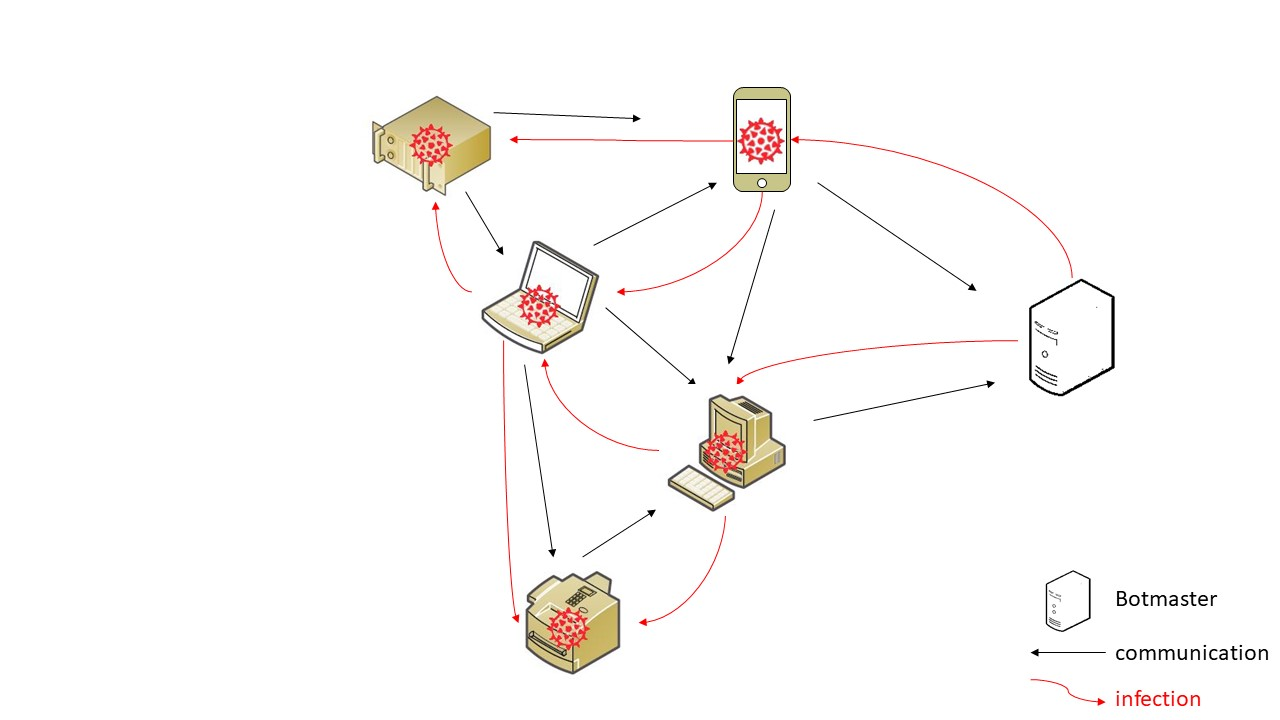
\includegraphics[width=0.75\textwidth]{P2P_non_structure}
	\label{fig:P2P_non_structure}
	\caption{P2P non structuré}
\end{figure}
\begin{figure}[h]
	\centering
		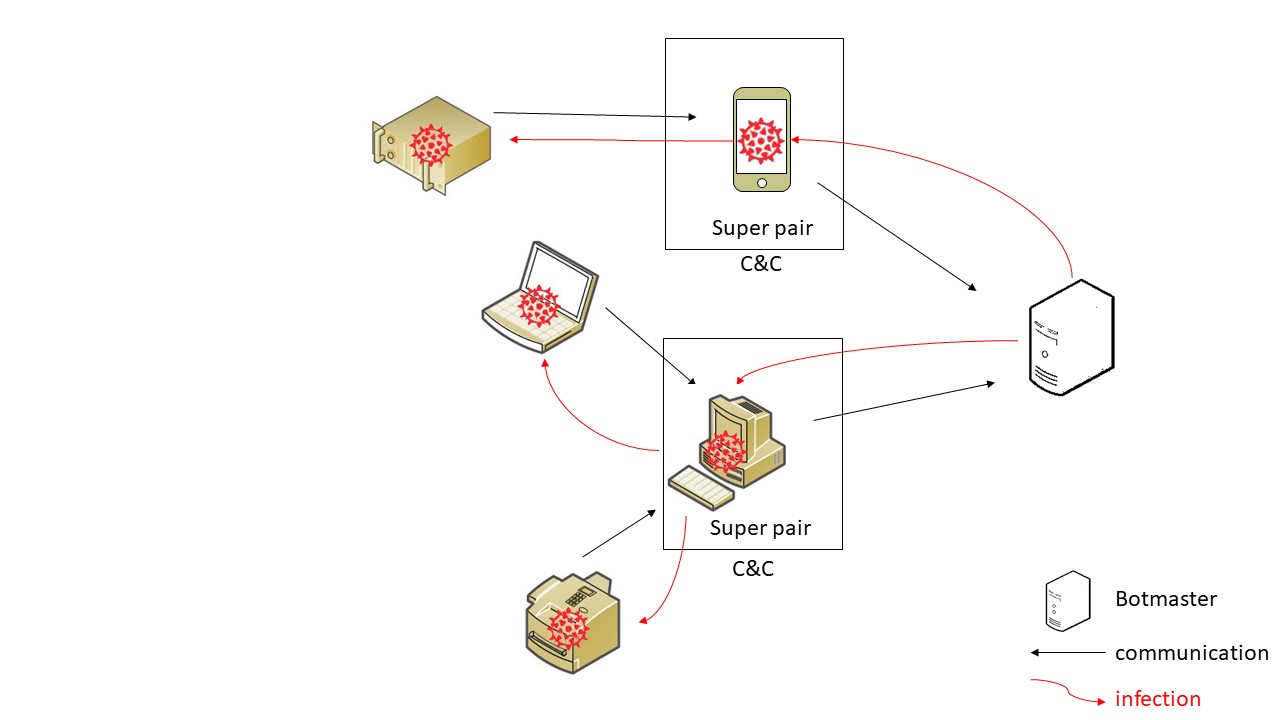
\includegraphics[width=0.75\textwidth]{P2P_avec_super_pairs}
	\label{fig:P2P_avec_super_pairs}
	\caption{P2P avec super-pairs}
\end{figure}

\subsubsection{Définition}
\par En utilisant des réseaux peer-to-peer, on s’affranchit d'un point central de communication.Chaque bot, selon ses caractéristiques, apporte les ressources pour élaborer le système de C\&C.
Il existe plusieurs typologies de réseau overlay\footnote{réseau logique de recouvrement}:
\begin{itemize}
	\item \textbf{overlay P2P non-structuré} : les topologies sont aléatoires (loi de puissance, aléatoire uniforme,...)
  \item \textbf{overlay P2P par super-pairs} : tous les pairs du réseau ne sont pas égaux, certains d’entre eux étant automatiquement sélectionnés pour servir temporairement le rôle de serveur pour les recherches ou le contrôle du réseau (comme FastTrack ou Gnutella)
  \item \textbf{overlay P2P structuré} : une cartographie établissant le lien entre le contenu et son emplacement ; ce type de réseau implémente en général – mais pas systématiquement une table de hachage distribuée (DHT) ; on retrouve dans cette catégorie les protocoles P2P Chord, Tapestry et Kademlia (utilisé par le logiciel eMule).
\end{itemize}

\subsubsection{Liste des protocoles utilisés par le botnet}
\begin{itemize}
	\item TCP/IP
	\item UDP
\end{itemize}

\subsubsection{Avantages}
\begin{itemize}
	\item Architecture dé centraliséee
	\item Indépendant de l’architecture DNS
	\item difficile à repérer
	\item Connexions régulières entre les bots et le C\&C (non permanente)
	\item Le botmaster donne les informations comme un bot faisant partie du réseau
  \item L’information transite de voisin en voisin
	\item très difficile à neutraliser
\end{itemize}

\subsubsection{Inconvénients}
\begin{itemize}
	\item Pas de vision globale du réseau par un bot
	\item Connexion en permanence
	\item Facile à détecter (filtrage du flux IRC)
\end{itemize}

%--------------------------------------------------------------------
%ajouter un botnet
%glisser le .csv dans le dossier exemples de la section 2
%inclure la ligne \csvautotabular[respect all]{Section/2-Ssection/exemples/nom-du-botnet}
%--------------------------------------------------------------------

\subsubsection{exemples}
\noindent
\resizebox{\textwidth}{!}{
\csvautotabular[respect all]{Section/2-Ssection/exemples/Storm.csv}
}
\resizebox{\textwidth}{!}{
\csvautotabular[respect all]{Section/2-Ssection/exemples/QAKBOT.csv}
}